\documentclass[11pt,a4paper]{scrbook}
\usepackage[utf8]{inputenc}
\usepackage{amsmath}
\usepackage{amsfonts}
\usepackage{amssymb}
\usepackage{graphicx}
\usepackage{longtable}
\usepackage{multirow}
\renewcommand{\familydefault}{\sfdefault}
\usepackage{droid}
\usepackage[left=2cm, right=1.5cm, top=2cm, bottom=1cm]{geometry}
\usepackage{ngerman}
\usepackage{tabularx}
\usepackage{graphicx}
\usepackage{enumitem}
\usepackage{scrpage2}	%Kopf- und Fußzeile
\usepackage{picinpar}	%Textumläufe von Grafiken
\usepackage{pdfpages}	%Implementierung von pdf als ganze Seite(Seiten sind nicht editierbar)
\usepackage{lastpage}	%Implmentiert 'letzte Seite', wird für Kopfzeile benötigt
\usepackage{listings}
%\usepackage{hyperref}

\usepackage{lastpage}



\pagestyle{scrheadings}
\ifoot{\ } \setfootsepline{1pt}\ofoot{ \thepage \  von \pageref{LastPage}\ }

\headsep=4.5cm 
\footskip=0.5cm
\textheight =22.3cm
\ihead{



\raggedleft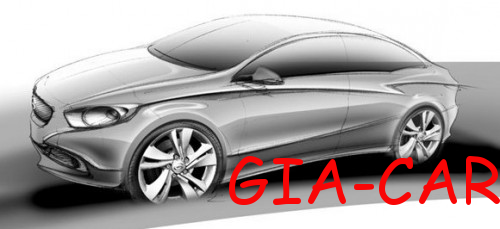
\includegraphics[width=0.3\linewidth]{./images/GIAcar.png}
\begin{tabular}{p{8cm} p{1.5cm} p{1.5cm} p{1cm} p{3.5cm}}
  \tabularnewline
  \textbf{Protokoll} &     &     & Suthe  &  \today\tabularnewline 
  \hline
\end{tabular}
}

%\ifoot{\ } \setfootsepline{1pt}\ofoot{ \\ }

\begin{document}

\section*{26.01.2017}
\textbf{Allgemeine, aktuelle Infos:}
\begin{itemize}
\item URL-Webserver: gc.antim8.de
\end{itemize}
\section*{02.02.17}
\Large{Darstellung der erarbeiteten Ergebnisse}
\normalsize
\begin{itemize}
\item Benedikt und Carlo: \\
Planung des Logins, Anzeigendarstellung, mit Warenkorb
Klassendiagramm zum Login (mit Hand)
\item Quang: \\
Design für die Startseite
\item Bjarne und Max: \\
erstellen Login - Funktionsweise: Benutzername gia  Passwort:  car\\
Login per php für die Webseite. Das Login schützt das komplette Projekt vor öffentlichen Zugriffen
\item Simon und Daniel: \\
ERD erstellt\\
Datenbank angelegt nach ERD \\
php-Code für Verbindung Webseite und Datenbank
Kommunikation zwischen Bjarne/Daniel und Benedikt für das Kundenlogin notwendig
\item Sebastian und Martin
Martin und Sebastian stellen das Sequenzdiagramm vor.
\item Planung des weiteren Vorgehens:
Zwei Personen planen das Klassendiagramm, dieses wird den anderen Klassenmitgliedern vorgestellt. Anhand des Klassendiagramms werden die Aufgaben für die Programme geplant.
\end{itemize}
\vspace*{1cm}
\Large{Aufgabenverteilung}
\normalsize
\begin{itemize}
\item Bjarne, Simon, Daniel: Datenbank
\item Benedikt, Carlo: Klassendiagramm
\item Max, Noah: Datenbank online erreichbar (Schnittstelle zur Webseite)
\item Quang, Martin, Sebastian : Design, Gestaltung und Funktion der Automobilseiten, Anpassung des Frameworks
\end{itemize}
\newpage
\vspace*{1cm}
\Large{festgelegte Details:}
\normalsize
\begin{itemize}
\item Kaufprozess:
\begin{itemize}
\item 0 = verfügbar
\item 1 = reserviert
\item 2 = bezahlt
\item 3 = ausgeliefert
\end{itemize}

\end{itemize}

\vspace*{1cm}
\Large{Aufgaben zum nächsten Mal}
\normalsize
\begin{itemize}
\item Suthe, Carlo, Benedikt: Klassendiagramm zu ende
\item Quang, Martin und Sebastian: Design
\item Simon, Daniel, Bjarne: Datenbank- / Controllerergänzung
\item Max, Noah: php-myadmin, User anlegenn
\end{itemize}





\end{document}




